\documentclass[11pt,aspectratio=169,usenames,dvipsnames]{beamer}
\usetheme{SimplePlus}

\usepackage{threeparttable}
\usepackage{booktabs}
\usepackage{xcolor} % For custom colors
\usepackage{tikz} % For styling enumerate numbers
\usepackage{tcolorbox} % For colored box styling
\usepackage{amsmath, amsfonts, amssymb, amsthm} % Math related
\usepackage{natbib}
\usepackage{fontspec}
\usepackage{luatexja}
\usepackage[mathscr]{euscript}
% ---------------- %
% color definition %
% ---------------- %
\definecolor{main}{HTML}{23373B}
\definecolor{pink}{RGB}{180, 50, 110}
\definecolor{orange}{HTML}{FF8000}
\definecolor{red}{HTML}{990000}
\definecolor{blue}{HTML}{004C99}
\definecolor{lightgray}{HTML}{E7E7E7}
\definecolor{gray}{RGB}{90, 90, 90}

\usepackage{hyperref}
\hypersetup{
     colorlinks   = true,
     linkcolor    = blue,
     citecolor    = blue
}


\newcommand{\pink}[1]{\textcolor{pink}{#1}}
\newcommand{\orange}[1]{\textcolor{orange}{#1}}
\newcommand{\red}[1]{\textcolor{red}{#1}}
\newcommand{\blue}[1]{\textcolor{blue}{#1}}
\newcommand{\green}[1]{\textcolor{OliveGreen}{#1}}
\newcommand{\magenta}[1]{\textcolor{magenta}{#1}}
\newcommand{\gray}[1]{\textcolor{gray}{#1}}
\newcommand{\purple}[1]{\textcolor{purple}{#1}}
\definecolor{yellow}{HTML}{EDB120}

% \setbeamercolor{alerted text}{fg=blue}

%%% automatically add spaces into enumerate and itemize environment
\let\tempone\itemize
\let\temptwo\enditemize
\renewenvironment{itemize}{\tempone\addtolength{\itemsep}{\fill}}{\temptwo}
\let\tempa\enumerate
\let\tempb\endenumerate
\renewenvironment{enumerate}{\tempa\addtolength{\itemsep}{\fill}}{\tempb}

\usepackage{fontawesome5}
\setbeamertemplate{itemize item}{\faAngleRight}
\setbeamertemplate{itemize subitem}{\faAngleDoubleRight}

\setmainfont{Crimson Pro Light}[
  ItalicFont={* Italic},
  BoldFont={Crimson Pro Medium},
  BoldItalicFont={Crimson Pro Medium Italic}]
\setsansfont{Crimson Pro Light}[
  ItalicFont={* Italic},
  BoldFont={Crimson Pro Medium},
  BoldItalicFont={Crimson Pro Medium Italic}]

\usepackage[mode=tex]{standalone}
\usepackage{tikz}
\usetikzlibrary{decorations}
\usetikzlibrary{decorations.pathreplacing, intersections}
\usepackage{pgfplots}
\usetikzlibrary{calc,positioning}
\usepgfplotslibrary{fillbetween}
\pgfplotsset{compat=newest, scale only axis, width = 10cm}

% --------------------------- %
% Section title page with toc %
% --------------------------- %
\setbeamertemplate{subsection page}{%
    \usebeamertemplate*{section page}
}
\setbeamertemplate{section in toc}[square]
\setbeamertemplate{subsection in toc}[square]
\AtBeginSection[]{
% \sepframe
\begin{frame}[noframenumbering]{Outline}
    % \tableofcontents[currentsection]
    \tableofcontents[currentsection, currentsubsection]
\end{frame}
}
\AtBeginSubsection[]{
  \begin{frame}[noframenumbering]{Outline}
    \tableofcontents[currentsection, currentsubsection]
  \end{frame}
}

% ------------ %
% beamerbutton %
% ------------ %
\newcommand{\goto}[2]{\hyperlink{#2}{\beamergotobutton{#1}}}
\newcommand{\return}[2]{\hyperlink{#2}{\beamerreturnbutton{#1}}}
\newcommand{\extgoto}[2]{\href{#2}{\beamergotobutton{#1}}}

\hypersetup{
    pdfpagemode=UseNone,
    pdftitle = {Macroeconomics I, Lecture 3},
    pdfauthor = {Hui-Jun Chen},
    pdfsubject = {},
    pdfkeywords = {},
}
\title[Lecture 1]{Lecture 3: \\Business Cycle Measurement}
\author[Hui-Jun Chen]{Hui-Jun Chen}
\institute{National Tsing Hua University}
\date{\today}

\begin{document}

% Title Page
\begin{frame}[plain]
    \titlepage
\end{frame}

\section{Math Concept}
\label{sec:Math_Concept}

\begin{frame}{Review: Trend and Cycle in Per Capital Real GDP}
\label{slide:Review__Trend_and_Cycle_in_Per_Capital_Real_GDP}
\begin{columns}
    \begin{column}{0.5\textwidth}
        \begin{figure}
            \caption{Figure 1.3: Natural log of Per Capita Real GDP and trend, 1900–2014: \alert{$y = \ln(Y)$, trend = HPFilter(y)}}
            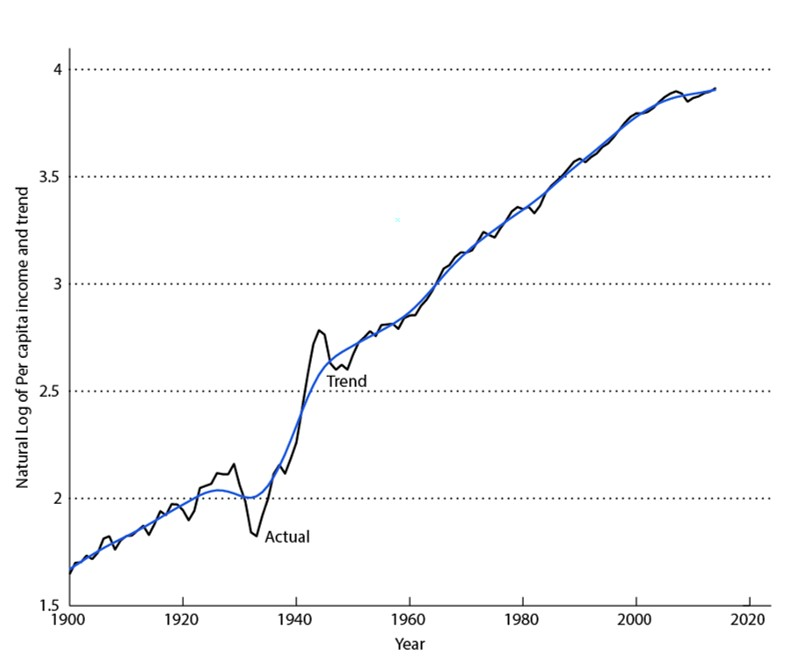
\includegraphics[width=\textwidth]{./figures/Figure1_3.jpg}
        \end{figure}
    \end{column}
    \begin{column}{0.5\textwidth}
        \begin{figure}
            \caption{Figure 1.4 Percentage Deviation from Trend in Per Capita Real GDP: \alert{actual - trend}}
            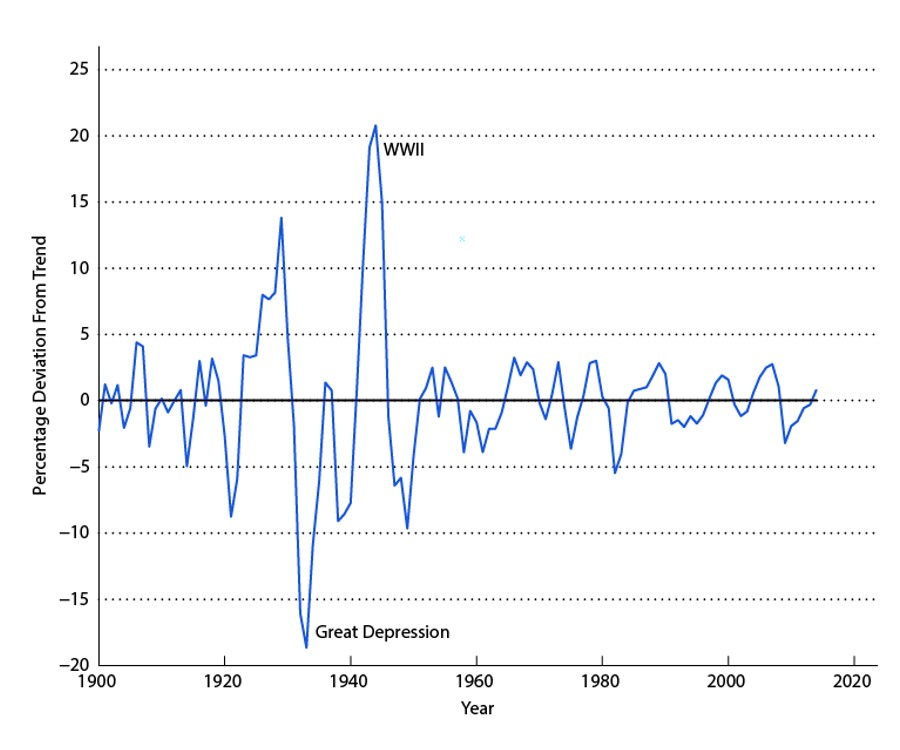
\includegraphics[width=\textwidth]{./figures/Figure1_4.jpg}
        \end{figure}
    \end{column}
\end{columns}
\begin{center}
    How do we measure the fluctuation?
\end{center}
\end{frame}

\begin{frame}{Statistical Concept to measure fluctuation}
\label{slide:Statistical_Concept}
    \begin{itemize}
        \item \textbf{mean/average} $ \bar{X} $: average level of variable $ X $
        %
        \begin{equation}
        \label{eq:average}
            \bar{X} = E( X ) \approx \frac{1}{N} \sum_{i=1}^{N} X_{i}
        ,\end{equation}
        %
        e.g. $ X = \{ 1, 2, 3, 4, 5 \} $, $ \bar{X} = \frac{1+2+3+4+5}{5} = 3 $
        \item \textbf{variance} $ \sigma_{X}^{2} $: dispersion of variable $ X $ relative to mean
        %
        \begin{equation}
        \label{eq:variance}
            \sigma_{X}^{2} = V( X ) = E[ ( X - \bar{X} )^{2} ] \approx \frac{1}{N} \sum_{i=1}^{N} [ ( X_{i} - \bar{X} )^{2} ]
        ,\end{equation}
        %
        e.g. $ \sigma_{X}^{2} = \frac{( 1-3 )^{2} + ( 2-3 )^{2} + ( 3-3 )^{2} + ( 4-3 )^{2} + ( 5-3 )^{2}}{5} = \frac{4 + 1 + 0 + 1 + 4}{5} = 2  $

        \textbf{standard deviation} is $ \sigma_{X} = \sqrt{\sigma_{X}^{2}} $.

    \end{itemize}
\end{frame}

\begin{frame}{Statistical Concept to measure fluctuation (Cont.)}
\label{slide:Statistical_Concept_to_measure_fluctuation__Cont__}
    \begin{itemize}
        \item \textbf{covariance} $ \sigma_{XY} $: dispersion of variable $ X $ ``associates'' with $ Y $.
        %
        \begin{equation}
        \label{eq:covariance}
            \sigma_{XY}
                = E[ ( X - \bar{X} ) ( Y - \bar{Y} ) ]
                \approx \frac{1}{N} \sum_{i=1}^{N} [ ( X_{i} - \bar{X} ) ( Y_{i} - \bar{Y} ) ]
        ,\end{equation}
        %
        e.g. $ Y = \{ 2, 3, 4, 5, 6 \} $, $ \bar{Y} = 4 $, $ \sigma_{XY}
                = \frac{( 1-3 )( 2-4 ) + ( 2-3 )( 3-4 ) + ( 3-3 )( 4-4 ) + ( 4-3 )( 5-4 ) + ( 5-3 )( 6-4 )}{5} = 2$
        \item \textbf{correlation} $ \rho_{XY} $: level of association between variables $ X $ and $ Y $
        %
        \begin{equation}
        \label{eq:correlation}
            \rho_{XY} = \frac{\sigma_{XY}}{\sigma_{X} \sigma_{Y}}
        ,\end{equation}
        %
        e.g. $ \rho_{XY} = \frac{2}{\sqrt{2} \times \sqrt{2}} = 1$

        $ \rho_{XY} > 0 $: $ X $ and $ Y $ move \alert{together}; $ < 0 $: move \alert{opposite} directions
    \end{itemize}
\end{frame}

\section{Measure GDP \& comove}
\label{sec:Measure_GDP____comove}

\begin{frame}{GDP Fluctuations: Definition and Measurement}
\label{slide:GDP_Fluctuations__Definition_and_Measurement}
    \begin{columns}
        \begin{column}{0.5\textwidth}
            \begin{itemize}
                \item \textbf{Business cycle}: fluctuations about trend in real GDP
                \item \textbf{Booms/Expansions}: persistent \alert{positive} deviation
                \item \textbf{Recessions}: persistent \alert{negative} deviation
                \item \textbf{Peak/Trough}: turning points on deviations
                \item \textbf{Amplitude}: size of deviations
                \item \textbf{Frequency}: \# of peaks per year
            \end{itemize}
        \end{column}
        \begin{column}{0.5\textwidth}
            \begin{figure}
                \caption{Figure 3.1 Business Cycle}
                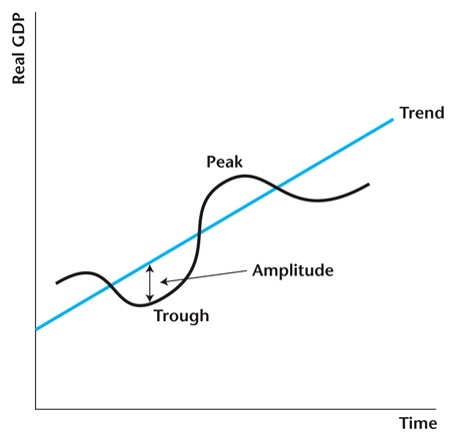
\includegraphics[width=.85\textwidth]{./figures/Fugre3_1.jpg}
            \end{figure}
        \end{column}
    \end{columns}
\end{frame}


\begin{frame}{Measurement on Comovement}
\label{slide:Measurement_on_Comovement}
    Three key concepts to measure comovement of variables $ X $ with GDP $ Y $:
    \begin{enumerate}
        \item \textbf{relative volatility} $ \sigma_{X} / \sigma_{Y} $: how noisy is $ X $ relative to GDP
        \begin{itemize}
            \item $ \sigma_{X} / \sigma_{Y} $ high $ \Rightarrow  $ $ X $ is noisy
        \end{itemize}
        \item \textbf{cyclicality} $ \rho_{XY} $: how does $ X $ comove with GDP?
        \begin{enumerate}
            \item \alert{procyclical}: $ \rho_{XY} > 0 $, $ X $ and GDP comove \alert{together}
            \item \alert{acyclical}: $ \rho_{XY} \approx 0 $, $ X $ and GDP not comoving
            \item \alert{countercyclical}: $ \rho_{XY} < 0 $, $ X $ and GDP move in \alert{opposite} direction
        \end{enumerate}
        \item \textbf{lead/coincident/lag}: does $ X $ predict GDP (lead), the opposite (lag) or nor (coincident)?
    \end{enumerate}
\end{frame}

\section{Visualization}
\label{sec:Visualization}

\begin{frame}{Visualization of Correlation: Scatter Plots}
\label{slide:Visualization_of_Correlation__Scatter_Plots}
    \begin{figure}
        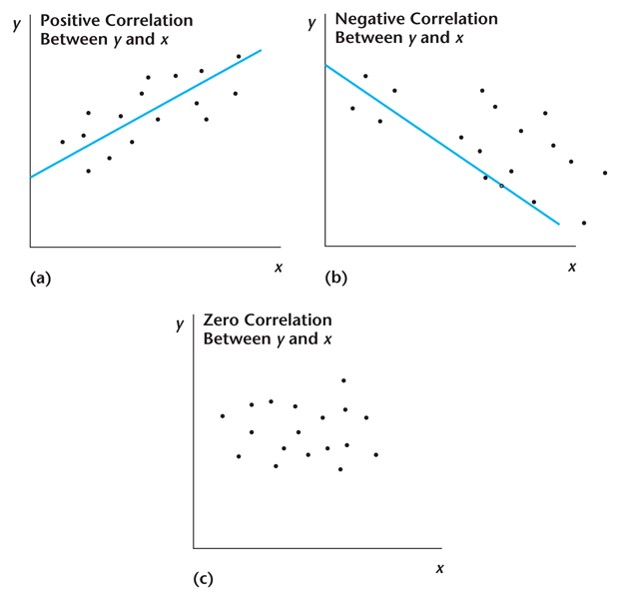
\includegraphics[width=0.5\textwidth]{./figures/Figure3_4.jpg}
    \end{figure}
\end{frame}

\begin{frame}{Visualization of Correlation: Time Series}
\label{slide:Visualization_of_Correlation__Time_Series}
    \begin{figure}
        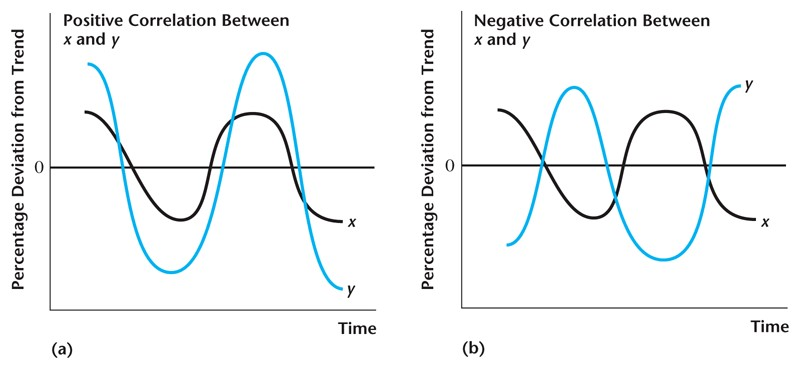
\includegraphics[width=\textwidth]{./figures/Figure3_3.jpg}
    \end{figure}
\end{frame}

\begin{frame}{Visualization of Leading and Lagging: Time Series}
\label{slide:Visualization_of_Leading_and_Lagging__Time_Series}
    \begin{figure}
        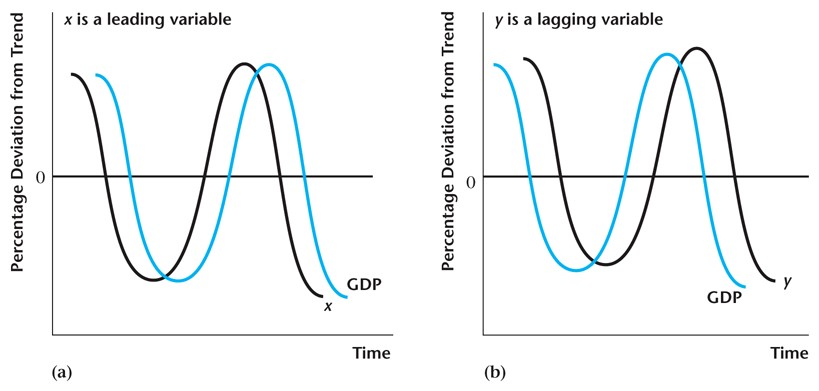
\includegraphics[width=\textwidth]{./figures/Figure3_7.jpg}
    \end{figure}
\end{frame}


\section{Data}
\label{sec:Data}

\begin{frame}{Data: Comovement of $ C $ and $ I $}
\label{slide:Data__Comovement_of___C___and___I__}

\begin{columns}
    \begin{column}{0.5\textwidth}
        \begin{figure}
            \caption{Figure 3.9 Percentage Deviations from Trend in \alert{Real Consumption} and Real GDP}
            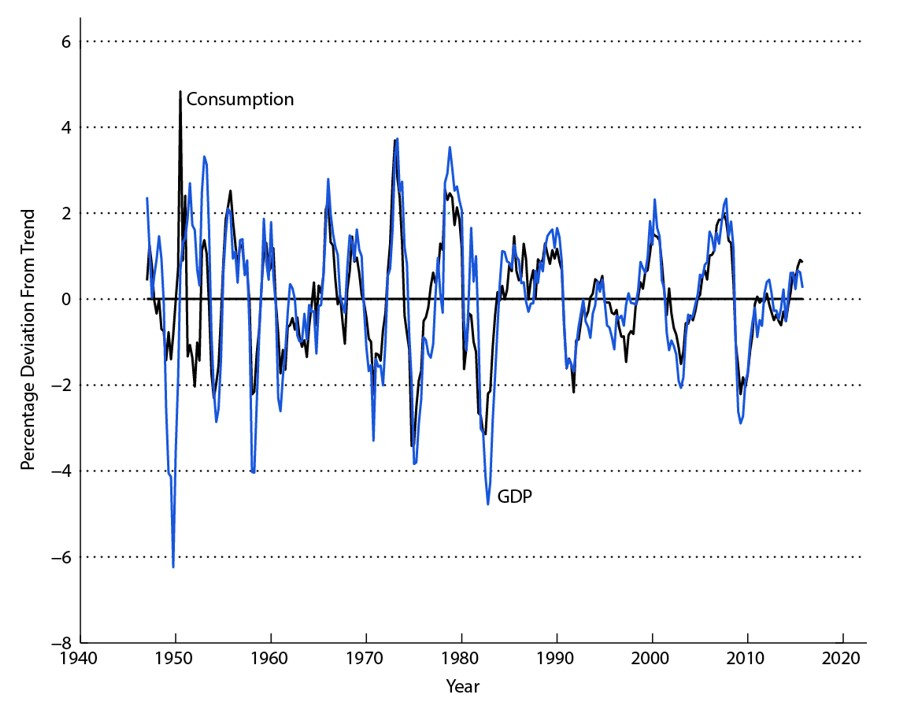
\includegraphics[width=\textwidth]{./figures/Figure3_9.jpg}
        \end{figure}
    \end{column}
    \begin{column}{0.5\textwidth}
        \begin{figure}
            \caption{Figure 3.10 Percentage Deviations from Trend in \alert{Real Investment} and Real GDP}
            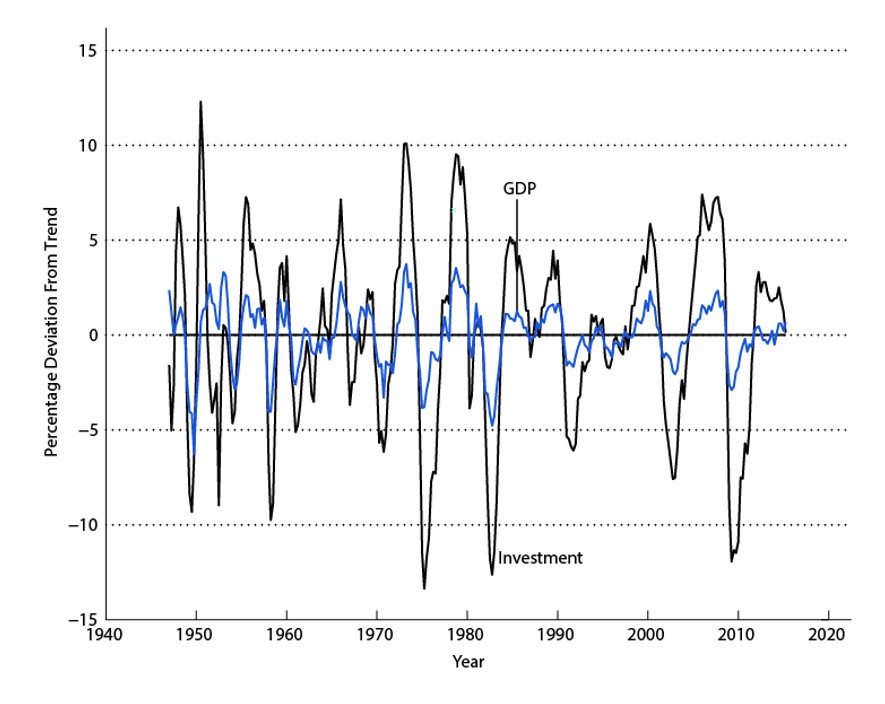
\includegraphics[width=\textwidth]{./figures/Figure3_10.jpg}
        \end{figure}
    \end{column}
\end{columns}
\end{frame}

\begin{frame}{Data: Correlation of Imports}
\label{slide:Data__Correlation_of_Imports}
    \begin{columns}
        \begin{column}{0.5\textwidth}
            \begin{figure}
                \caption{Figure 3.5  Time Series (Detrended)}
                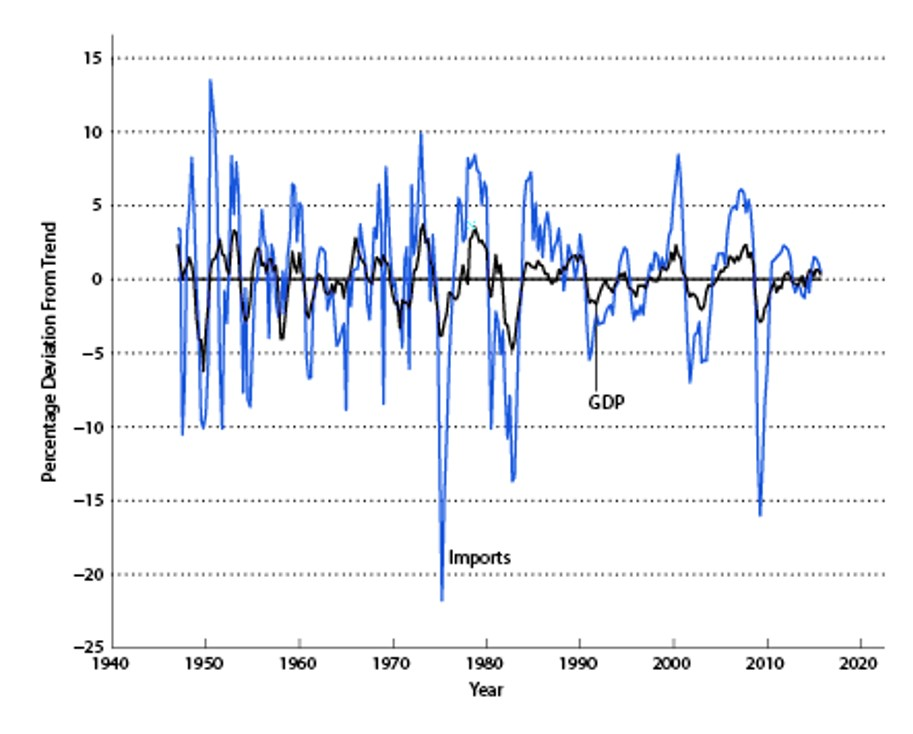
\includegraphics[width=\textwidth]{./figures/Figure3_5.jpg}
            \end{figure}
        \end{column}
        \begin{column}{0.5\textwidth}
            \begin{figure}
                \caption{Figure 3.6  Scatter Plot: Time Series}
                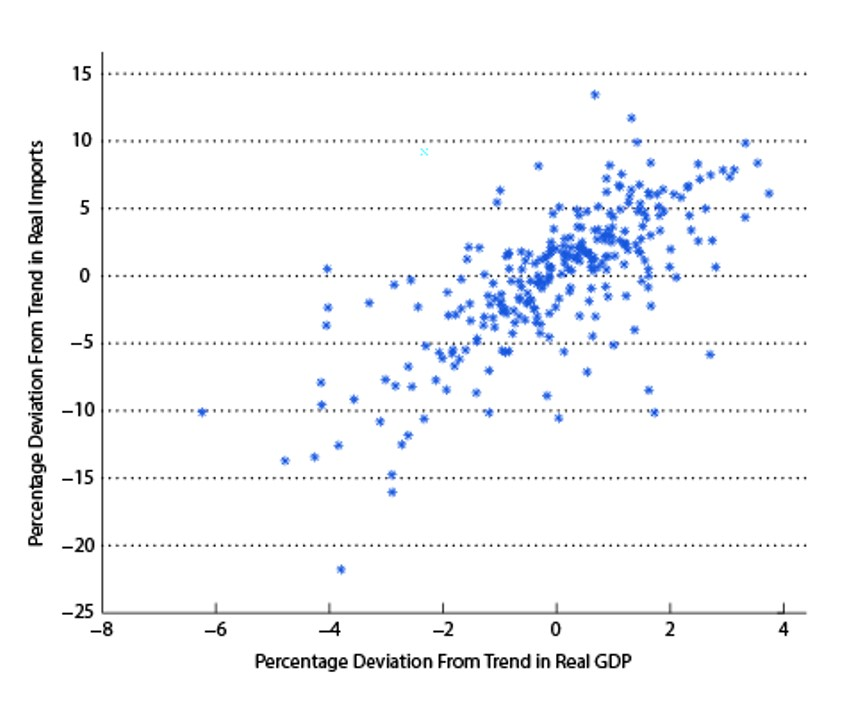
\includegraphics[width=\textwidth]{./figures/Figure3_6.jpg}
            \end{figure}
        \end{column}
    \end{columns}
\end{frame}

\begin{frame}{Data: Leading Indicator, Housing Starts}
\label{slide:Data__Leading_Indicator}
    \begin{columns}
        \begin{column}{0.5\textwidth}
            \begin{figure}
                \caption{Figure 3.8  Percentage Deviations in Real GDP and Housing Starts}
                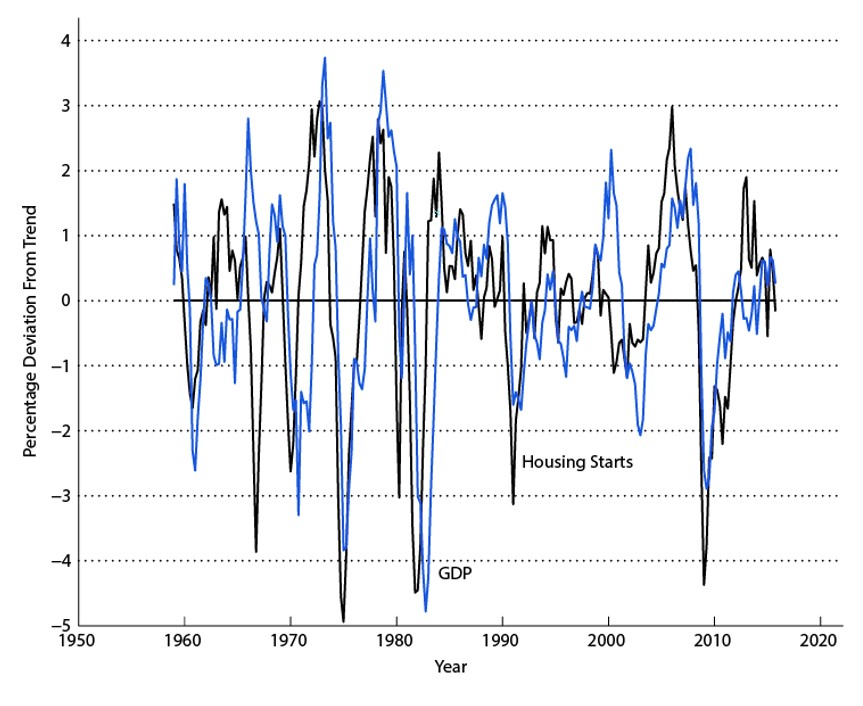
\includegraphics[width=\textwidth]{./figures/Figure3_8.jpg}
            \end{figure}
        \end{column}
        \begin{column}{0.5\textwidth}
            \begin{itemize}
                \item \textbf{Def}: the construction project is started for a private dwelling
                \item \alert{Question}: Why housing start is predicting GDP?
                \item Ans: \alert{commitment} to a quantity of residential \alert{investment}
            \end{itemize}
        \end{column}
    \end{columns}
\end{frame}

\begin{frame}{Summary}
\label{slide:Summary}

\begin{table}[h!]
\caption{Business cycle statistics relative to GDP}
\centering
\scalebox{0.9}{
\begin{tabular}{|l|c|c|c|c|c|}
\hline
\textbf{Variable} &
\textbf{Corr. Coef.} &
\shortstack{\textbf{Std Dev} \\ \textbf{(\% of S.D. GDP)}} &
\textbf{Cyclicality} &
\textbf{Lead/Lag} &
\shortstack{\textbf{Variation} \\ \textbf{Relative to GDP}} \\
\hline
consumption & 0.77 & 77  & Procyclical & Coincident & Smaller \\
\hline
investment  & 0.80 & 301 & Procyclical & Coincident & Larger  \\
\hline
employment  & 0.78 & 65  & Procyclical & Lagging   & Smaller \\
\hline
average labor productivity & 0.77 & 63  & Procyclical & Coincident & Smaller \\
\hline
\end{tabular}}
\end{table}
\end{frame}

% \appendix

% \begin{frame}[allowframebreaks]{References}
% \footnotesize
% \bibliographystyle{$BIB_STYLE}
% \bibliography{$BIBFILE}
% \end{frame}

\end{document}
